\chapter{Implementación y configuración en Visual Studio}
\section{Estructura del proyecto}
\begin{table}[H]
\centering
\caption{Archivos de entrada más relevantes}
\label{tab:files}
\begin{tabular}{P{4.8cm}P{10.0cm}}
\toprule
\thd{Archivo} & \thd{Responsabilidad observada}\\
\midrule
\texttt{TicTacToeMinMax\allowbreak.csproj} & Destino Android, identidad de aplicación, recursos e inclusiones de paquetes.\\
\texttt{MauiProgram.cs} & Construye la aplicación MAUI y agrega registro de depuración en configuración DEBUG.\\
\texttt{App.xaml.cs} & Crea la ventana principal con \texttt{AppShell}.\\
\texttt{AppShell.xaml} & Declara \texttt{MainPage} como contenido inicial.\\
\texttt{MainPage.xaml} & Define textos, tablero contenedor, botones, menús y estilos.\\
\texttt{MainPage.xaml.cs} & Coordina turnos, estado, eventos, reinicio, salida y resultados.\\
\texttt{UnbeatableAI}\allowbreak\texttt{Controller.cs} & Evalúa estados y busca el movimiento de \texttt{O}.\\
\texttt{AndroidManifest.xml} & Manifiesto y permisos Android declarados.\\
\texttt{launchSettings.json} & Incluye un perfil llamado \emph{Windows Machine}; no identifica el emulador Android.\\
\bottomrule
\end{tabular}
\end{table}

\section{Configuración comprobada}
La inspección del equipo y del proyecto encontró Visual Studio Community 2026 versión 18.11.0, SDK de .NET 10.0.402 y las cargas de trabajo de MAUI/Android 10.0.110. El proyecto usa MAUI con destino Android y mínimo de plataforma API 21. En la barra de Visual Studio se ve la configuración \emph{Debug}, \emph{Any CPU} y el destino seleccionado \emph{Pixel 7 -- API 36.0 (Android 16.0 -- API 36)}. Los requisitos de plataforma de MAUI para Android 5.0/API 21 o posterior coinciden con el valor mínimo del proyecto \cite{mauiPlatforms}.

\begin{table}[H]
\centering
\caption{Propiedades del proyecto y valores encontrados}
\label{tab:config}
\begin{tabular}{P{5.0cm}P{9.8cm}}
\toprule
\thd{Propiedad} & \thd{Valor observado}\\
\midrule
Target framework & \texttt{net10.0-android}\\
Tipo de salida & \texttt{Exe}\\
MAUI y proyecto único & \texttt{UseMaui=true}; \texttt{SingleProject=true}\\
Nullable reference types & Habilitado\\
Versión mínima Android & \texttt{SupportedOSPlatformVersion=21.0}\\
Título de aplicación & \texttt{Tic-Tac-Toe}\\
Application ID & \texttt{com.companyname.tictactoeminmax}\\
Versión de aplicación & \texttt{1.0}; versión numérica \texttt{1}\\
Icono e imagen de inicio & \texttt{Resources/AppIcon/appicon.png}; pantalla inicial blanca, base 128$\times$128\\
Imagen incluida & \texttt{Resources/Images/pic\_character.png}\\
Paquetes & \texttt{Microsoft.Maui.Controls} con \texttt{\$(MauiVersion)} y \texttt{Microsoft.Extensions.Logging.Debug} 10.0.0\\
\bottomrule
\end{tabular}
\end{table}

El proyecto incluye una sola plataforma en \texttt{TargetFramework}, aunque MAUI permita compartir código con otros destinos. El emulador seleccionado en Visual Studio es evidencia de configuración de depuración; no se interpreta como una ejecución nueva de la aplicación. El README de las capturas identifica el dispositivo usado para la evidencia anterior como \texttt{emulator-5554}; no se atribuye un número de serie a la selección mostrada por Visual Studio.

\section{Capturas de configuración en Visual Studio}
Las capturas se generaron desde la ventana de Visual Studio con el proyecto MAUI cargado. Se muestran el destino Android seleccionado y la configuración del archivo de proyecto; no se modificó el código para producirlas.

\begin{figure}[!htbp]
\centering
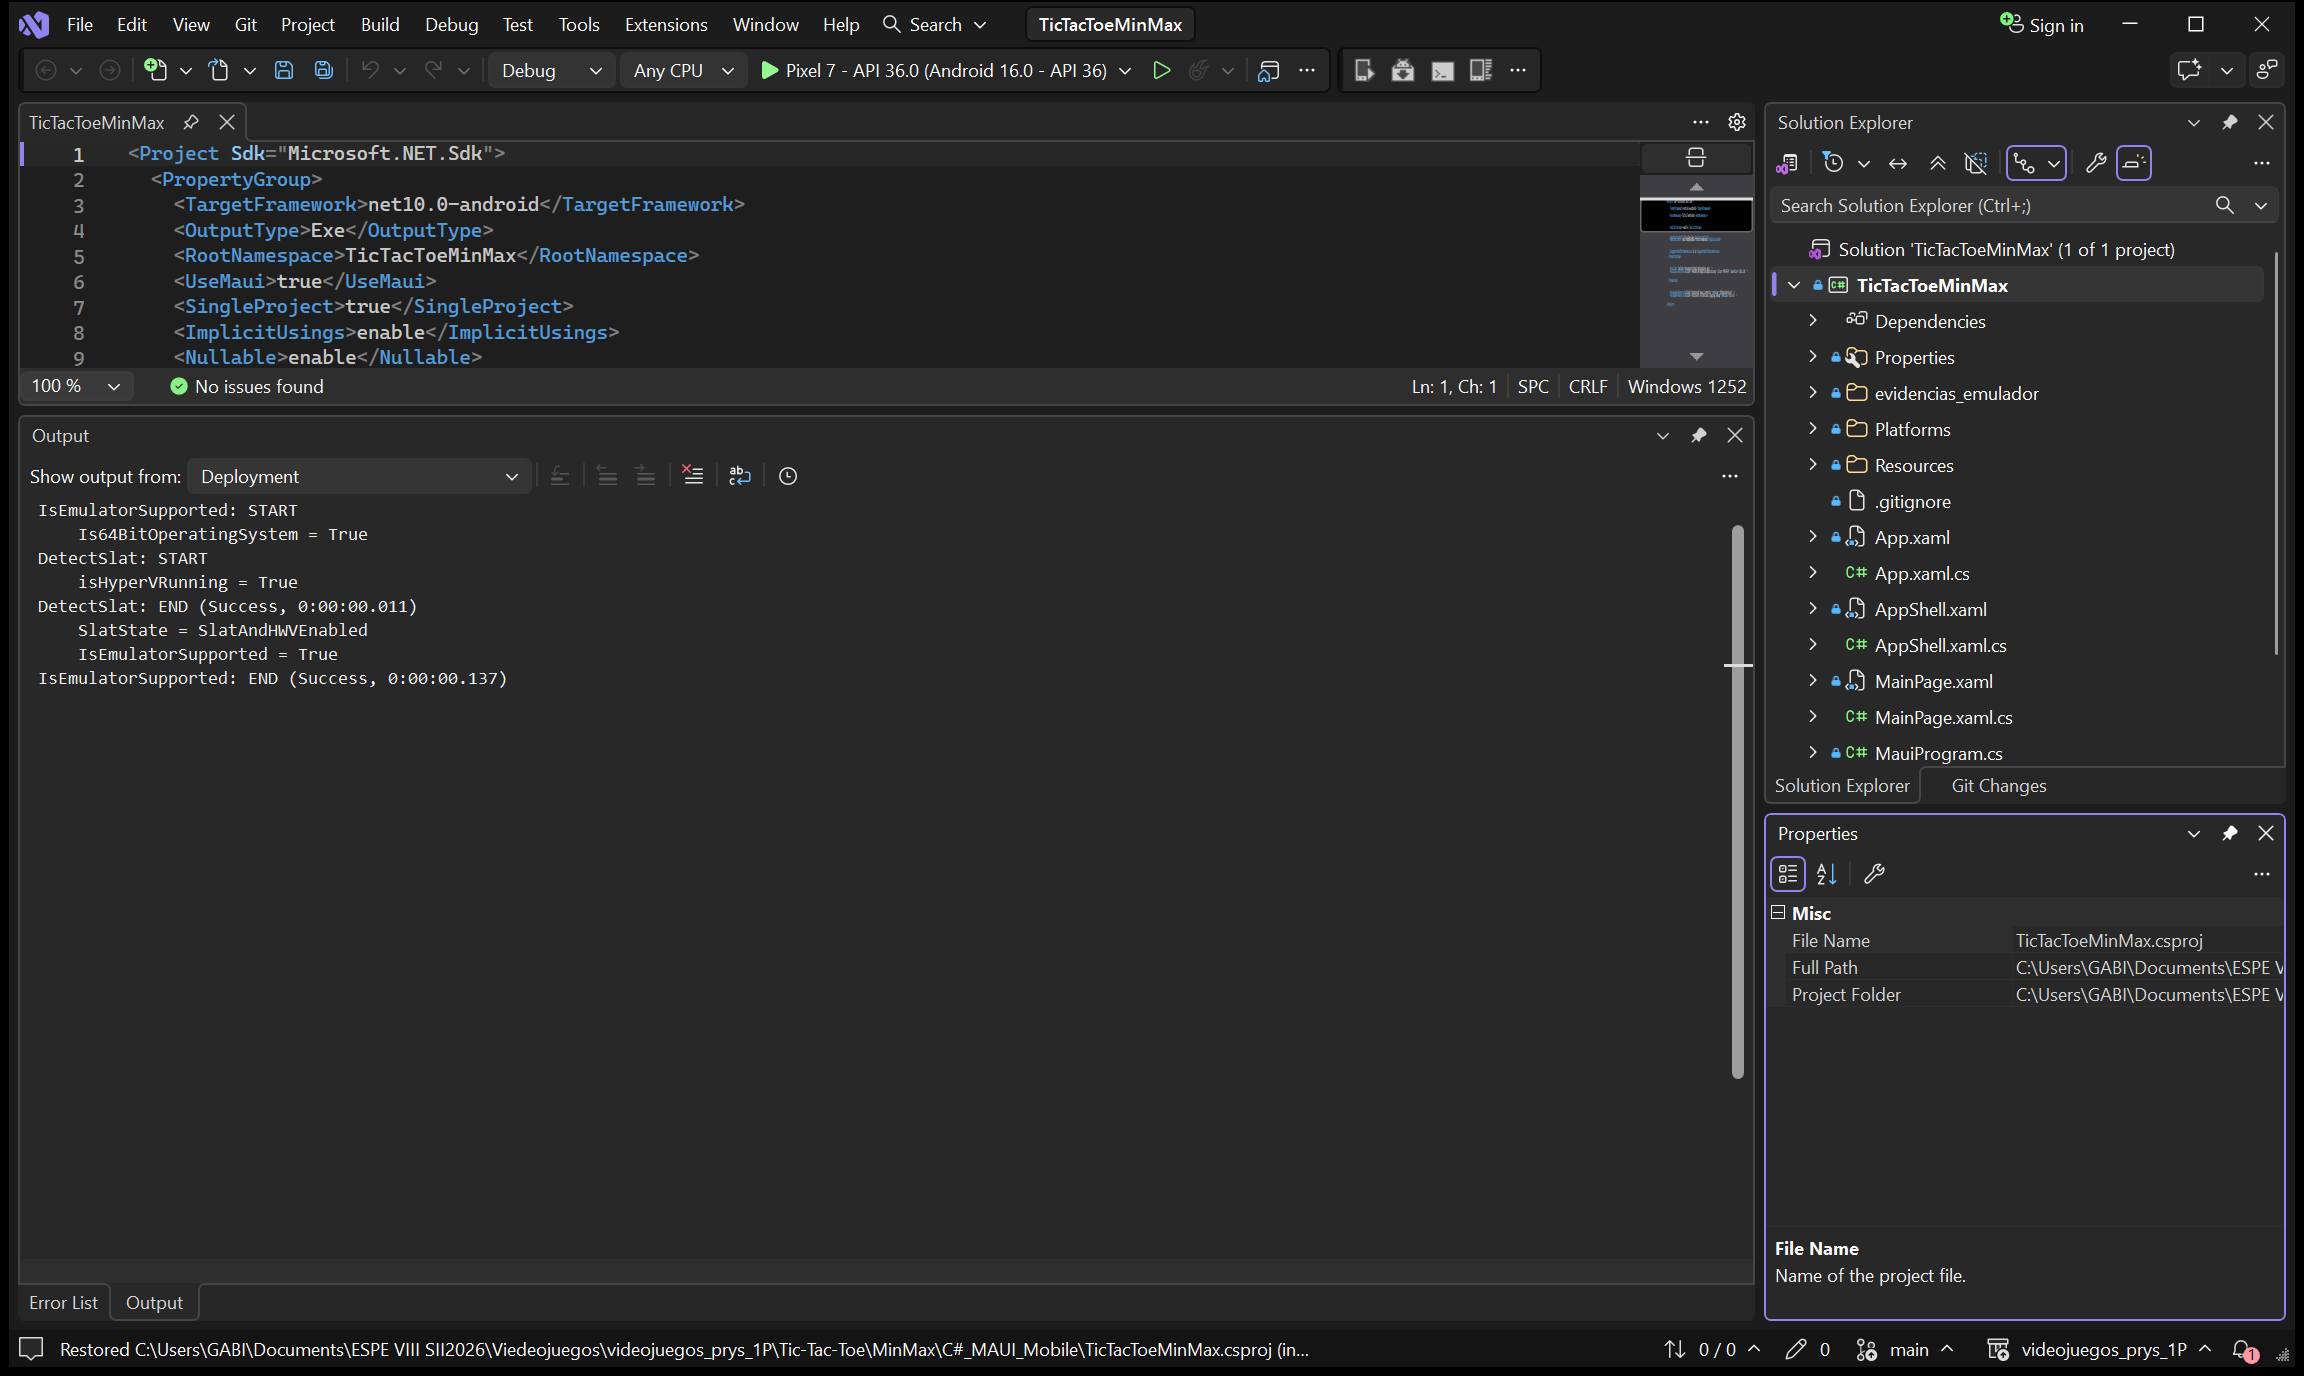
\includegraphics[width=\textwidth]{configuraciones_visual_studio/01_visual_studio_proyecto.png}
\caption{Visual Studio Community 2026 con el proyecto cargado. La barra muestra Debug, Any CPU y el emulador Android seleccionado; el editor muestra el destino \texttt{net10.0-android}.}
\label{fig:vs-project}
\end{figure}

\begin{figure}[!htbp]
\centering
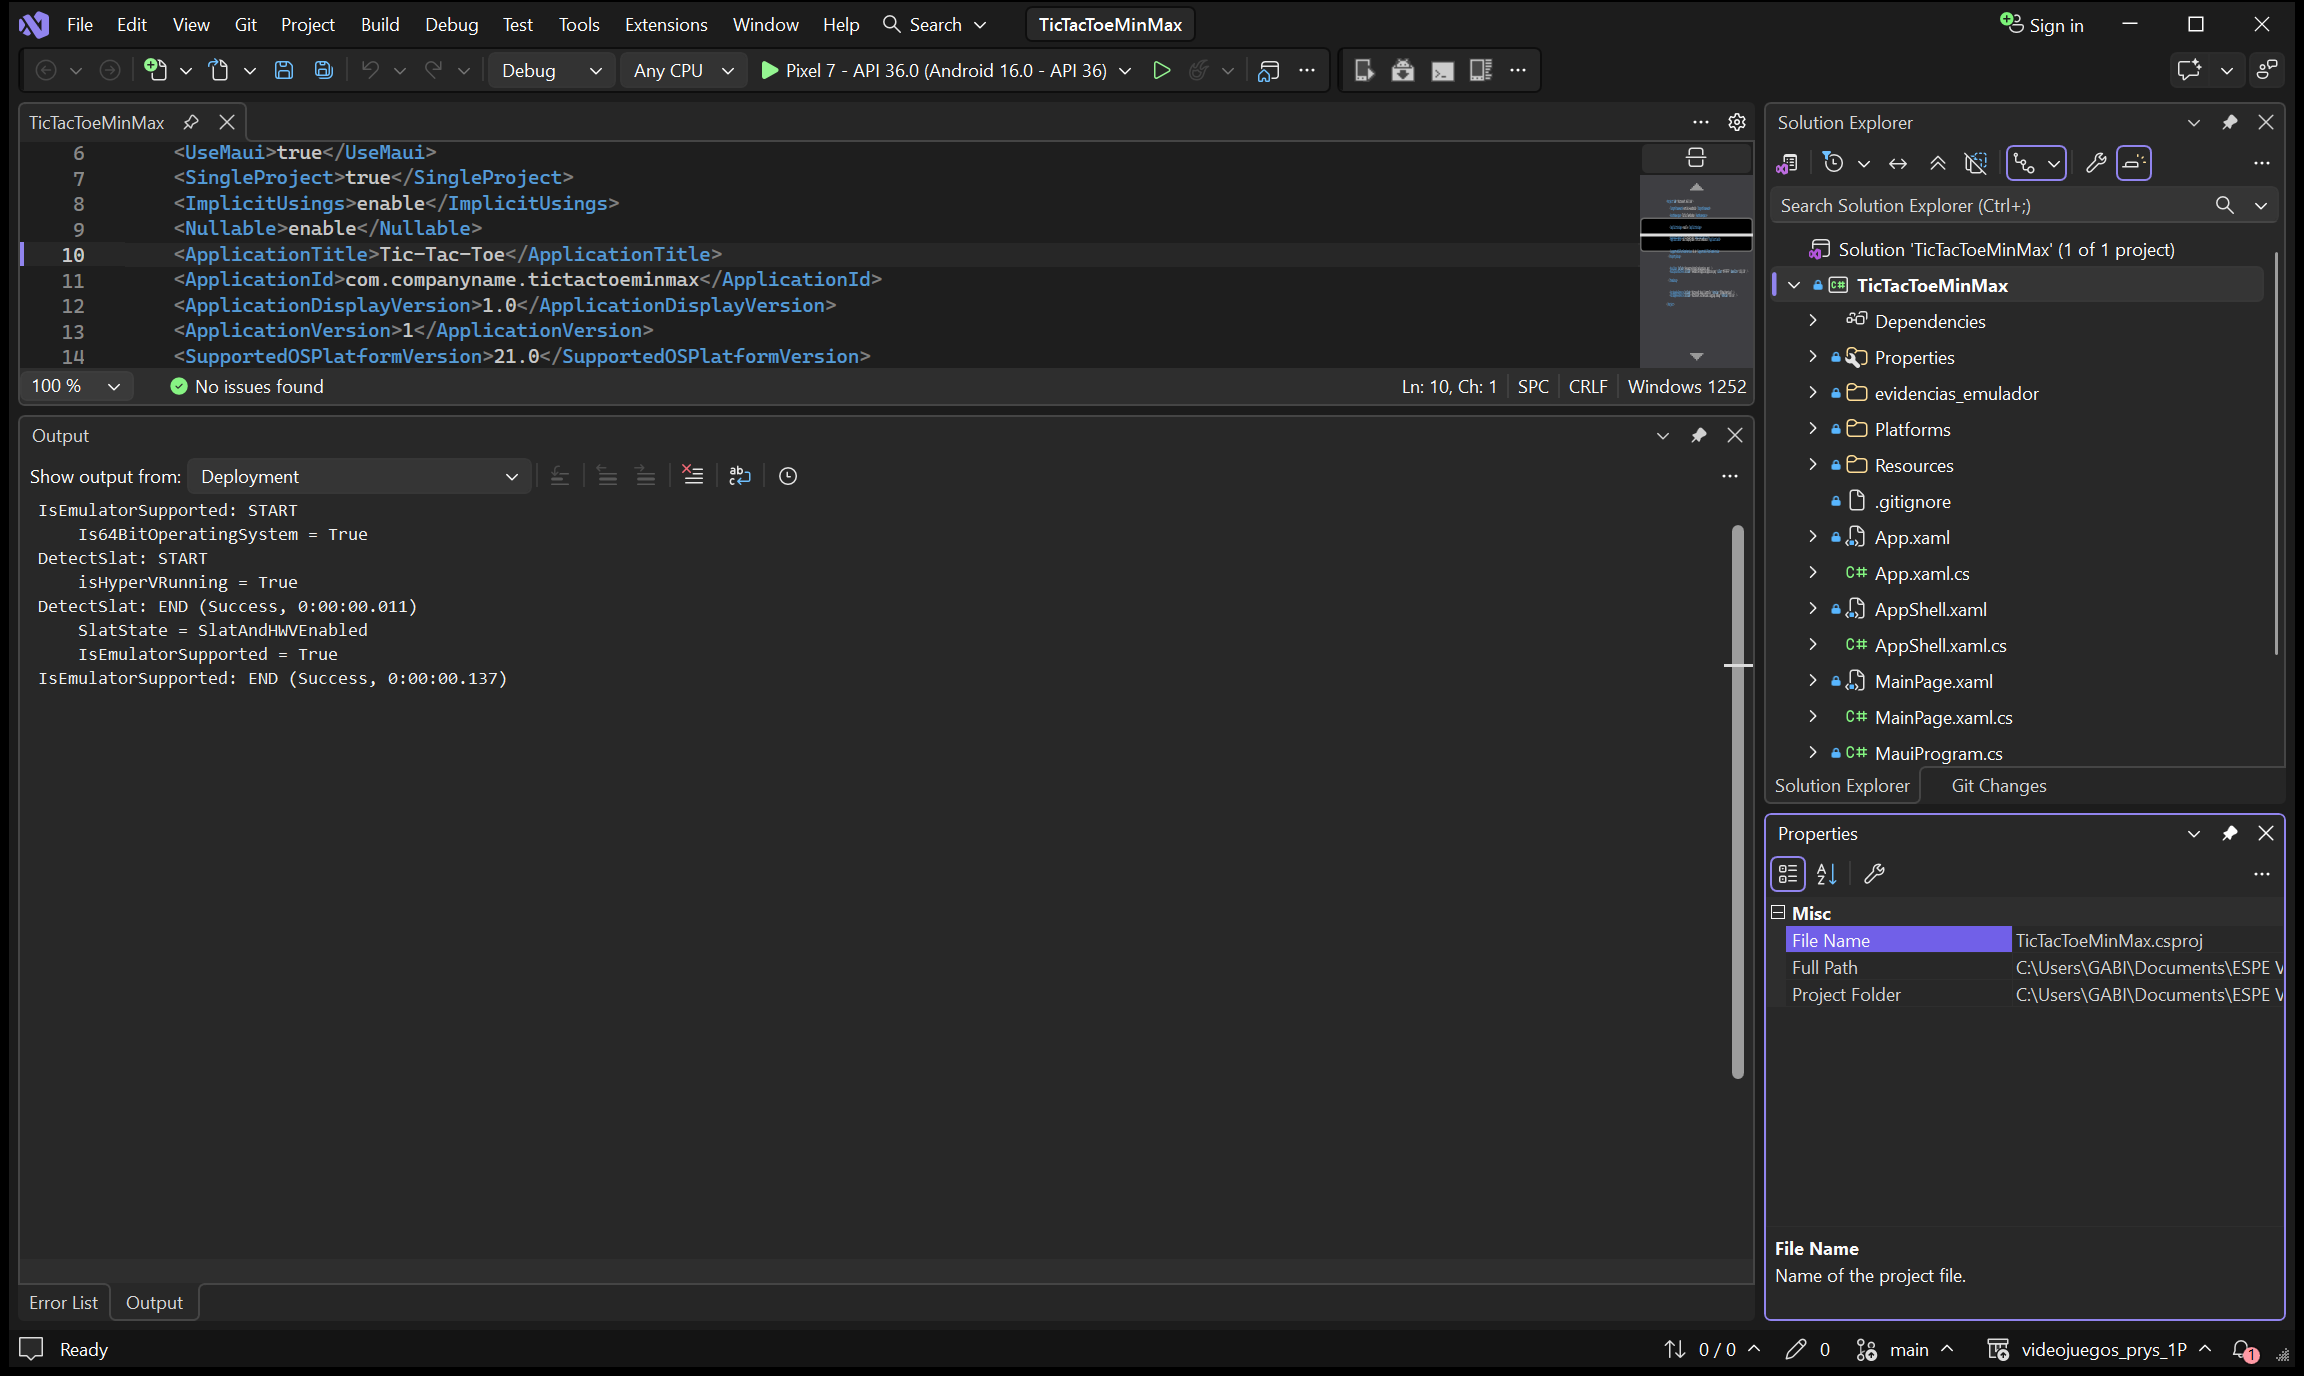
\includegraphics[width=\textwidth]{configuraciones_visual_studio/02_visual_studio_target_android.png}
\caption{Configuración de aplicación y plataforma en el \texttt{.csproj}: título, Application ID, versiones y mínimo Android API 21.}
\label{fig:vs-target}
\end{figure}

\begin{figure}[!htbp]
\centering
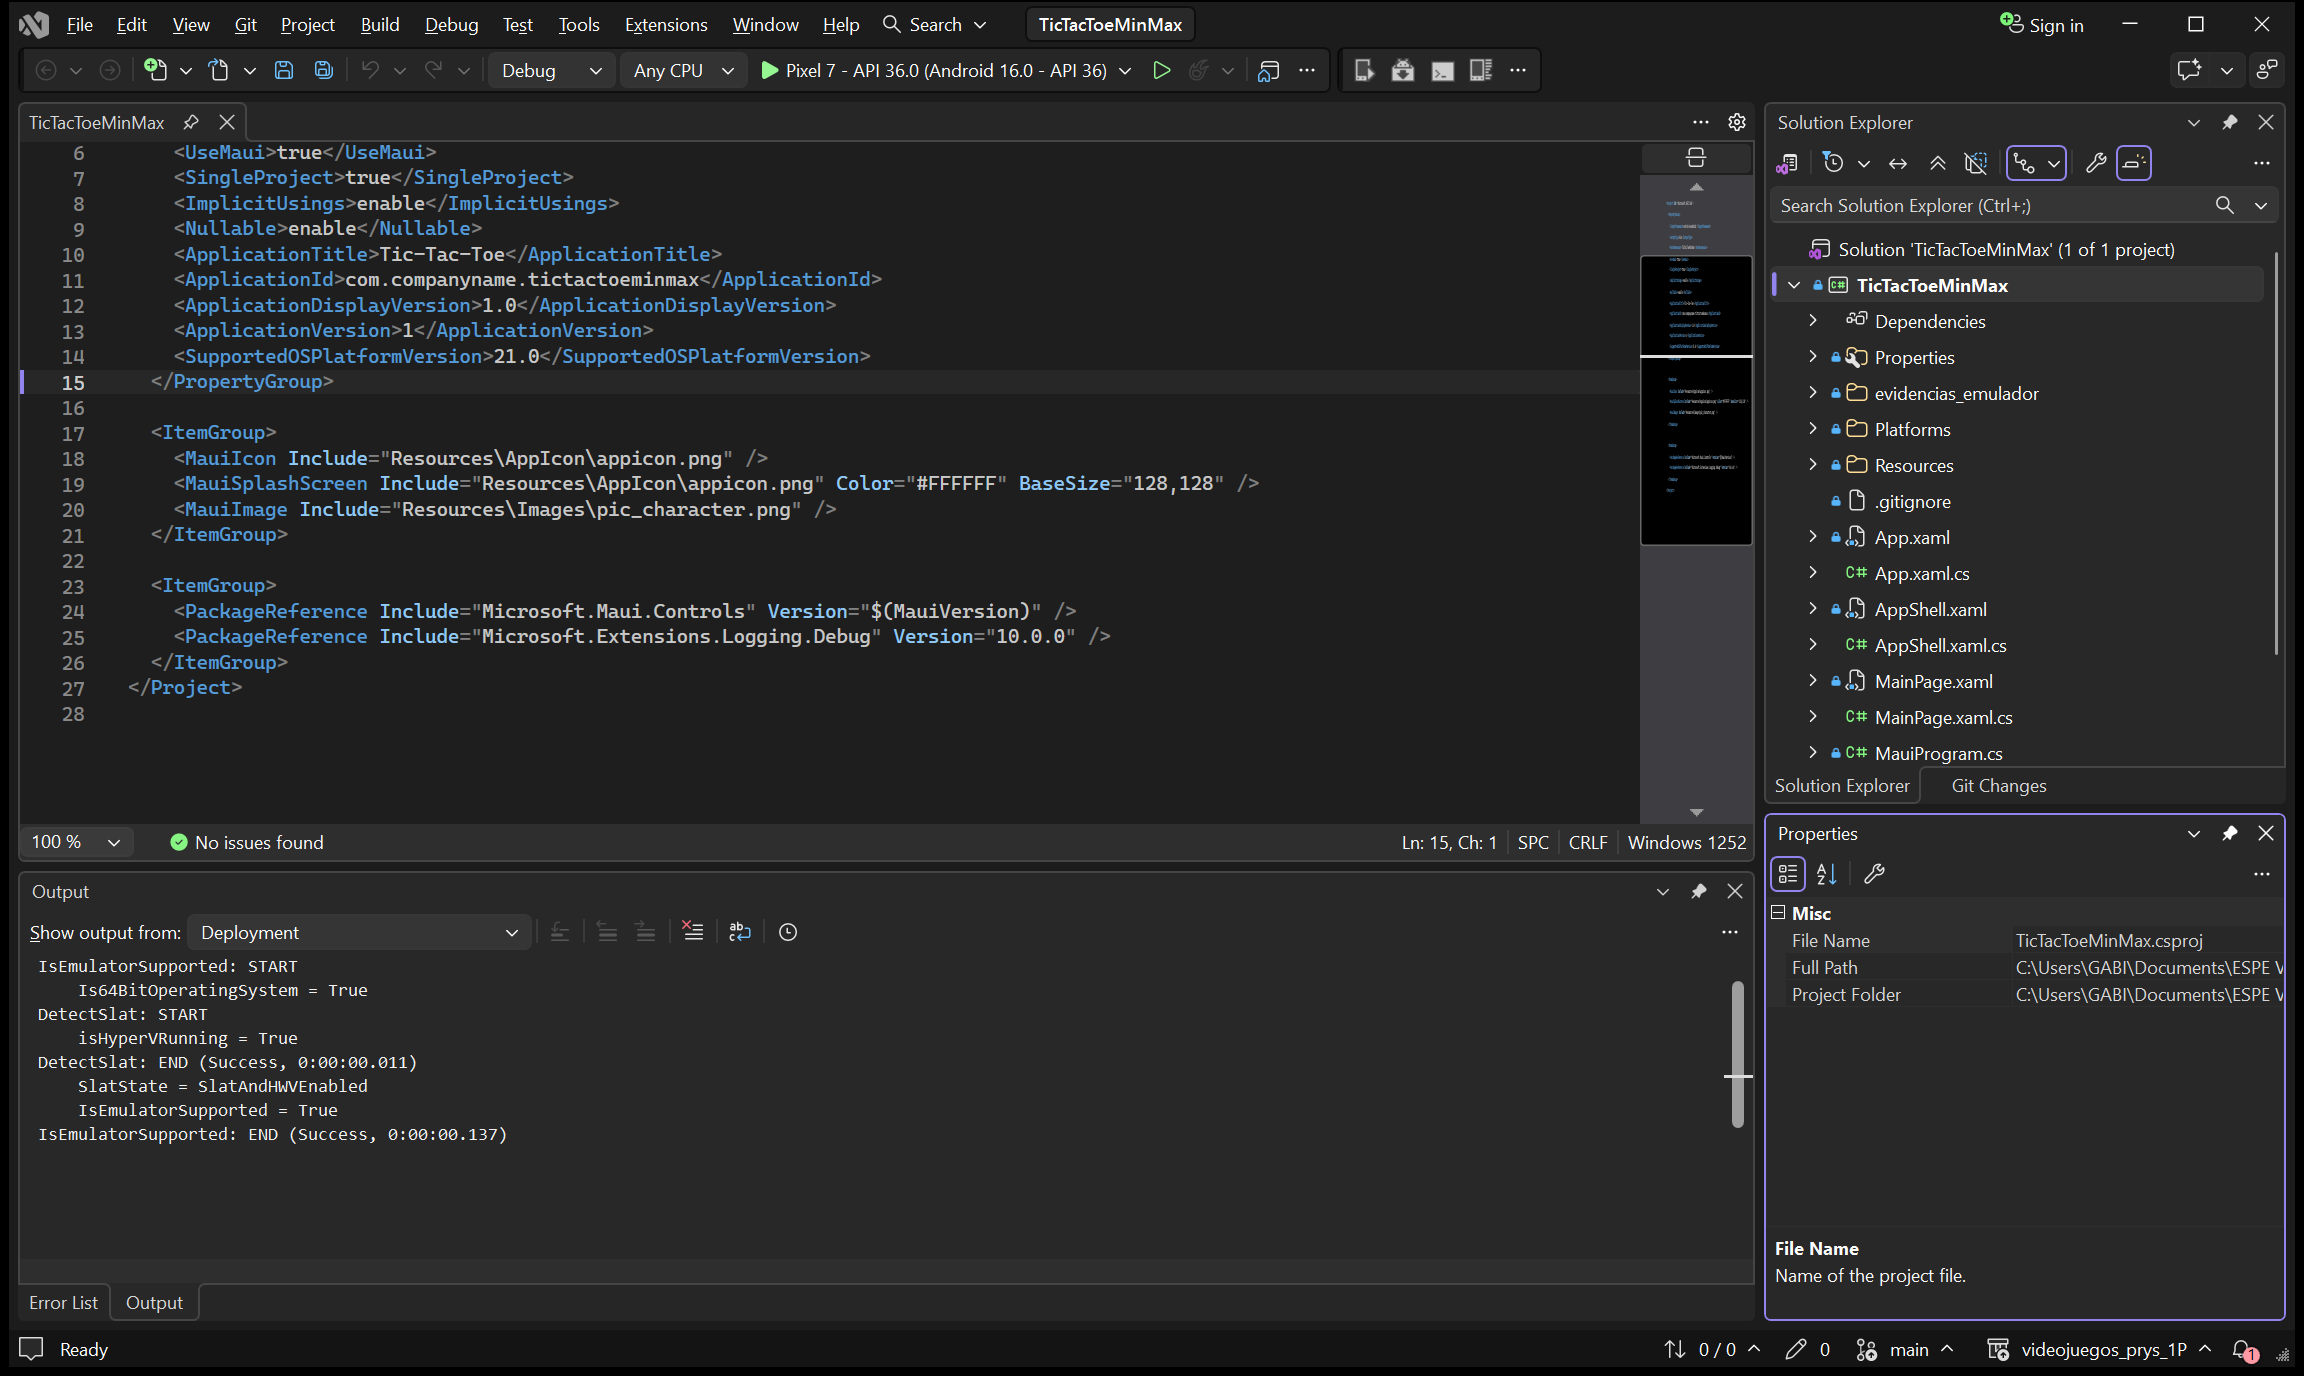
\includegraphics[width=\textwidth]{configuraciones_visual_studio/03_visual_studio_paquetes_recursos.png}
\caption{Recursos MAUI y referencias de paquetes declarados en el proyecto.}
\label{fig:vs-resources}
\end{figure}

\section{Pasos para abrir y ejecutar desde Visual Studio}
\begin{enumerate}
  \item Iniciar Visual Studio y escoger \textbf{Abrir un proyecto o una solución}.
  \item Seleccionar \ruta{TicTacToeMinMax.csproj} dentro de \ruta{Tic-Tac-Toe/MinMax/C\#\_MAUI\_Mobile}. El directorio no contiene un archivo de solución para este proyecto MAUI; se abre directamente el proyecto.
  \item Esperar la restauración de paquetes. Para desarrollar MAUI en Windows deben estar instalados el SDK de .NET MAUI y los componentes Android; Microsoft documenta su instalación desde Visual Studio Installer y la verificación mediante las cargas de trabajo instaladas \cite{mauiInstall}.
  \item En la barra de depuración, seleccionar \textbf{Debug}, \textbf{Any CPU} y un emulador Android. La captura de este equipo muestra \textbf{Pixel 7 -- API 36.0 (Android 16.0 -- API 36)}.
  \item Usar \textbf{Iniciar} o presionar \textbf{F5}. Si Visual Studio solicita un dispositivo, elegir un emulador Android disponible y esperar el despliegue.
  \item En la aplicación, tocar una casilla vacía. Comprobar que la persona juega con \texttt{X} y que la respuesta de Minimax aparece con \texttt{O}.
  \item Usar Nuevo para limpiar el tablero. La opción Salir cierra la aplicación; las opciones de los menús Archivo, Ver y Ayuda son solo presentacionales en la versión revisada.
\end{enumerate}

\section{Configuración Android que conviene conservar}
Las cargas de trabajo y el destino Android son coherentes con el archivo del proyecto. El perfil de \texttt{launchSettings.json} llamado \emph{Windows Machine} no describe el dispositivo Android; la selección del emulador se realiza desde la barra de depuración de Visual Studio. El manifiesto declara \texttt{INTERNET} y \texttt{ACCESS\_NETWORK\_STATE}; al no encontrarse uso de red en la lógica del juego, conviene justificar o retirar esos permisos en una revisión de configuración.

% ----------------------------------------------------------------------
